\section{Background} \label{sec:background}

In this chapter, we explain the essential concepts used in this thesis. We start by introducing \acl{dl} and its main aspects. Then, we present \aclp{cnn} and Autoencoders, two types of Deep Architectures used by the proposed method. In addition, an explanation of \acl{mtl} and its variants is presented. Later, we detail methods to explain Deep Networks, such as \acs{shap}, and for dimensionality reduction, like \acl{pca} and \acs{tsne}. Next, the metrics used to evaluate the proposed method are described in detail. Finally, the \icao standard is described, along with the \fvcongoing competition and its protocol.

\subsection{Deep Learning}

\acf{ai} is a study field of Computer Science focused on the design and construction of intelligent agent that receives inputs from the environment and take actions that affect that environemnt \citep{russell}. It can include, for example, learning, reasoning, and self-correction. In the early days of \acs{ai}, the first systems were heavily based on a set of rules previously provided by experts from certain subject areas. Usually, large rule-based problems are intellectually more difficult for humans than for computers; thus, machines can take advantage of them. Also, such systems have been developed for small and restricted environments. For example, we can cite Deep Blue \citep{hsu2002behind}, a successful chess-playing system developed by IBM that defeated the world champion Garry Kasparov in 1997.

As the scale and amount of data have increased over the years, traditional \acs{ai} methods have been replaced by a more data-driven approach called \acf{ml}. Instead of manually providing rules for the system, an algorithm automatically learns intrinsic patterns based on data. When the desired answers are also provided as inputs, we call it \textit{Supervised Learning}; otherwise, it is called \textit{Unsupervised Learning}. Many algorithms have been developed for both types of learning, for instance: Support Vector Machines \citep{boser1992training}, Decision Trees \citep{breiman1984classification}, and Mean Shift \citep{fukunaga1975estimation}. 

Although \acl{ml} represents an important advance in the \acs{ai} field, traditional algorithms are limited when processing raw data in their natural form (e.g., image pixels, text, or audio data). Typically, domain expertise is employed to carefully define how to extract useful features from raw data that can be used as inputs to the \acs{ml} algorithm. This process is usually referred to as feature engineering. However, it may be challenging for many tasks (for instance, detecting people in images) to define ``which'' and ``how'' features should be extracted.

Representation learning allows \acs{ml}-based systems to discover valuable representations from raw data automatically. According to \cite{goodfellow2016deep}, these learned representations often yield better performance in comparison to the hand-designed ones. Furthermore, representation learning algorithms enable \acs{ai} systems to adapt faster to new tasks with minimal human intervention.

\acf{dl} represents a particular sub-field of representation learning which allows computational models composed of multiple processing layers capable of learning data representations with many levels of abstraction \citep{lecun2015deep}. Therefore, complex representations can be obtained from a composition of simpler ones. For example, we can cite the problem of detecting faces in images. Mathematically defining a function that maps a set of pixels (raw format) into the desired output (face location) can be challenging. However, \acl{dl} can solve this problem by breaking the complex mapping into a series of simple nested mappings, each described by an individual model layer. For instance, the first layer may be responsible for detecting edges on raw pixels. Given these edge descriptions, the second layer may look for corners and contours since they are defined by a set of edges. Consecutively, the third layer can detect entire object parts (e.g., eyes, nose, and mouth) by identifying patterns in specific corners and contours. Finally, the parts of the object contained in the image can be evaluated to determine the presence (or absence) of the face in the image.

The most well-known examples of \acl{dl} models are \textbf{feedforward neural networks}, also called deep feedforward networks or multilayer perceptrons. They were inspired by the biological model of neurons, their connections, and how the human brain processes information. The quintessential unit of a feedforward neural network is a node (neuron) that receives the inputs of other nodes and computes an output. Each input is associated with a learnable parameter $w$ (synapse), also called \textbf{weight}, which assigns relative importance to the corresponding input. The weighted sum of the weights and inputs plus a \textbf{bias} compose the output of a neuron that is generally modified by an \textbf{activation function} responsible for introducing nonlinearity to the network. A stack of nodes at the same level forms a layer, and sequences of layers comprise the entire neural network. Each layer between the input and the output layer is called \textbf{hidden layer}. In a feedforward network, there are no feedback connections between the layers.

The set of weights and biases represents the trainable parameters of neural networks. Nevertheless, as with other \acs{ml} algorithms, neural networks have other types of parameters called \textbf{hyperparameters}. They are used to control the learning process and are commonly divided into two groups:

\begin{itemize}
\item \textbf{Model hyperparameters}: define aspects mainly related to the neural network architecture. For instance, we can cite the number of layers, the number of neurons in each layer, the activation function of each layer, momentum, dropout rate, and others.

\item \textbf{Training hyperparameters}: related to the learning process itself. For example, the cost function, number of epochs, optimizer, batch size, etc.
\end{itemize}

It is crucial to note that no optimal set of hyperparams can work for all kinds of particular problems, and their tuning is commonly performed manually. Also, while some hyperparams influence the time and memory cost to perform a prediction with the trained network, others affect the quality of the model and its capacity to output correct results when the network is presented to new inputs.

The rest of this section focuses on some specific types of neural networks and layers adopted in this thesis. Moreover, we describe a special kind of learning employed when networks may learn multiple tasks simultaneously, called \acl{mtl}.


\subsubsection{Convolutional Neural Networks}

\acfp{cnn}, also known as Convolutional Networks, are a specific kind of feedforward neural network specially developed to process grid-like data. For example, we can think of time-series data as a 1--D grid of time intervals with samples. Likewise, images can be considered as 2--D grid of pixels. In recent years, \acsp{cnn} have achieved exceptional performance in several practical applications. It includes, but is not limited to, image classification \citep{li2014medical, guo2017simple, paoletti2018new}, object detection \citep{cai2016unified, wu2017squeezedet}, and instance segmentation \citep{wang2020solov2, xu2020convolutional, zhang2020mask}.

The convolution is the basic operation of a \acs{cnn}. In summary, it is a well-known mathematical operation that performs a linear calculation over two functions \citep{goodfellow2016deep}. This is similar to the cross-correlation, but one of the functions is reversed and shifted. Given the functions $x$ and $w$, the convolution operation over an age of measurement $\tau$ between $x$ and $w$ - denoted by $h(t)$ - can be defined according to \autoref{eq:convolution}, for the continuous domain:

\begin{equation}
\label{eq:convolution}
h(t) = \int_{-\infty }^{\infty} x(\tau)w(t - \tau)\ d\tau
\end{equation}

\noindent
Typically, the convolution operation is expressed by an asterisk operator (\autoref{eq:conv_ast}):

\begin{equation}
\label{eq:conv_ast}
h(t) = (x * w)(t)
\end{equation}

\noindent
where $x$ represent the input, $w$ is the kernel, and $t$ is the point where the convolution is computed. If $w$ is a valid probability density function, the convolution can be considered a weighted average of the input at point $t$. Also, when working with discretized data (such as digital images), the \autoref{eq:convolution} can be rewritten as \autoref{eq:conv_discrete}:

\begin{equation}
\label{eq:conv_discrete}
h(t) = \sum_{\tau=-\infty}^{\infty} x(\tau)w(t - \tau)
\end{equation}

Usually, \acsp{cnn} are primarily applied to process images as inputs. In these cases, the input $x$ is represented by 4--D vectors, also called tensors, of $N \times H \times W \times C$ dimensions, where $N$ denotes the number of images in the dataset (samples), $H$ and $W$ are the image dimensions, and $C$ corresponds to the number of channels (e.g. colors) in each image. The kernel $w$ is also a multidimensional array that represents the parameters to be learned by the algorithm.

As pointed out by \cite{goodfellow2016deep}, convolution has three essential characteristics that help improve the performance of ML-based systems:

\begin{itemize}
\item \textbf{sparse interactions}: unlike dense neural networks, the output units do not need to interact with each input unit. Instead, the kernel $w$ is commonly smaller than the input. Therefore, fewer parameters must be stored, reducing the amount of memory and the number of operations the model requires, beyond improving its statistical efficiency.

\item \textbf{parameter sharing}: refers to reusing the same kernel across the whole image. In traditional neural nets, each weight is strictly applied only once to compute the output of a layer. However, in \acsp{cnn}, the weights presented in the kernel $w$ are applied to every image pixel (except, in some cases, for the boundary pixels or when  undersampling is employed - the stride hyperparameter). Therefore, convolutions are dramatically more effective than dense matrix multiplications.

\item \textbf{equivariant representations}: refers to the fact that convolutions are invariant to translations. A function is called equivariant when the output changes correspond to changes in the input. In mathematical terms, this implies that a function $f(x)$ is equivariant to the function $g$ if $f(g(x)) = g(f(x))$. In the case of convolutions, if $g$ is a function that shifts the input image, then the convolution output is translated by the same amount. This property helps detect specific patterns across an image, such as edges or even more complex shapes like faces. However, convolutions are not equivariant to transformations like image scaling or rotation.
\end{itemize}

In \aclp{cnn}, beyond the convolutional layers, there are also other common types of layers employed to perform distinct operations. Some other layers used in this work are described in the following subsections.

\paragraph{Pooling Layers}

Besides convolution, pooling layers are one of the essential components of \aclp{cnn}. Pooling is an operation that provides an approach to reduce the spatial size of feature maps, also called downsampling, and summarizes the features present in patches of the feature map. It helps to: (i) reduce the number of parameters; (ii) the number of computations performed in the network; and (iii) make the model more robust to slight variations in the position of features in the input image, controlling overfitting. In general, pooling layers are applied after the activation function of the convolutional layers and operate independently on each feature map.

There are two common types of pooling methods: \textbf{max pooling} and \textbf{average pooling}. They compute the maximum and the average value for each patch of a feature map, respectively. An example of both operations can be seen in \autoref{fig:poolings}.

\begin{figure*}[ht]
\centering
\subfigure[Max Pooling]{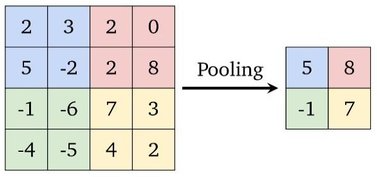
\includegraphics[width=0.4\linewidth]{images/deep_learning/pool_max.png}}
\hfill
\subfigure[Average Pooling]{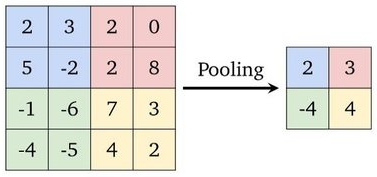
\includegraphics[width=0.4\linewidth]{images/deep_learning/pool_avg.png}}    
\caption{Example of Max Pooling and Average Pooling operations performed over a feature map of $4 \times 4$ with $pool\_size=2 \times 2$, $stride=2$, and no padding. Adapted from \citep{guissousallaeddine2019}.}
\label{fig:poolings}
\end{figure*}

The pooling layer has three input parameters: filter size (or pool size), stride, and whether to apply padding to the input image. Commonly, the filter size is $2 \times 2$, the stride is 2, and no padding is applied. Using this configuration, the feature map is reduced by half in each dimension, and 75\% of the original activations are discarded. The number of channels in the feature map (depth) remains unchanged.

There is a particular type of pooling known as \textbf{global pooling}, introduced by \cite{lin2013network}. In addition to the traditional method, the global version extends the pooling across the entire feature map. Therefore, if a given feature map has $H \times W \times C$ dimensions, it will be reduced to $1 \times 1 \times C$. Again, the most common functions used in global pooling are maximum and average. As stated by \cite{zhou2016learning}, such a difference makes the global pooling layers perform better in practice than the conventional approach. Moreover, it can substitute the flattened layers in the transition between convolutional layers and the fully connected network responsible for outputting a prediction.

Since pooling computes a fixed function of the input, no learning parameters are required by the pooling layers in Convolutional Networks. This is valid for all the pooling approaches described above (max, average, and global pooling).


\paragraph{Batch Normalization Layers}

Training \aclp{dnn} can be challenging due to many factors. For example, we can cite the random weights initialization, optimization algorithm, and chosen hyperparameters configuration. Furthermore, during the learning phase, each parameter is updated by the gradient under the assumption that the other layers do not change \citep{goodfellow2016deep}. However, in practice, all weights are updated simultaneously.

Another significant factor is related to the expectations around layer distributions. During training, the distribution of each layer's input changes as previous layers' parameters also change. This is referred to as Internal Covariate Shift \citep{ioffe2015batch}. It may cause unintended effects in the training of deep networks since small changes in shallower layers will be amplified during a forward pass to deeper hidden layers.

Batch Normalization is a regularization technique proposed by \cite{ioffe2015batch} to mitigate the effect of Internal Covariate Shift. It normalizes the inputs of hidden layers by using the first (mean) and second (variance) statistical moments of the current batch. This normalization step is usually applied before the activation function but can also be employed after the nonlinear function. The batch normalization makes the training of deep neural networks faster, more stable, and less likely to overfit. Also, batch normalization may substitute Dropout as a regularization technique.

Given a mini-batch $B$ $\{x_i, \ldots, x_m\}$ of size $m$, the mean and variance of $B$ are denoted by Equations \ref{eq:bn_mean} and \ref{eq:bn_stddev}, respectively:

\begin{equation}
\label{eq:bn_mean}
\mu_B = \frac{1}{m} \sum_{i}^{m} x_i
\end{equation}

\begin{equation}
\label{eq:bn_stddev}
\sigma_B^2 = \frac{1}{m} \sum_{i=1}^{m} (x_i - \mu_B)^{2}
\end{equation}

Subsequently, the input $x_i$ is normalized by \autoref{eq:bn_norm}:

\begin{equation}
\label{eq:bn_norm}
\hat{x}_i = \frac{x_i - \mu_B}{\sqrt{\sigma_B^{2} + \epsilon}}
\end{equation}

\noindent
where $x_i$ can be either the input or output of the activation function from the current layer and $\epsilon$ is an arbitrarily small constant added for numerical stability. The final output $y_i$ of the current layers is given by \autoref{eq:bn_output}:

\begin{equation}
\label{eq:bn_output}
y_i = \gamma\hat{x}_i + \beta
\end{equation}

\noindent
where $\gamma$ and $\beta$ are new learnable parameters introduced by batch normalization. 

One crucial aspect to highlight is that the network can automatically avoid batch normalization operations. That is, if the network during training converges to $\gamma=1$ and $\beta=0$, it means that the input $x_i$ does not need to be normalized; thus, the input $x_i$ remains unchanged.

During the training phase, the normalization steps are computed based on mini-batches to ensure reliable and efficient training. On the other hand, during inference, the network is generally asked to perform predictions for a given sample. For this reason, the normalization step is performed with the estimated population statistics. The population mean and variance are estimated during training and defined by Equations \ref{eq:bn_pop_mean} and \ref{eq:bn_pop_var}, respectively: 

\begin{equation}
\label{eq:bn_pop_mean}
E[x] = E_B[\mu_B]
\end{equation}

\begin{equation}
\label{eq:bn_pop_var}
Var[x] = \frac{m}{m-1} E_B[\sigma_B^{2}]
\end{equation}

Therefore, during inference, the input $x$ is normalized by \autoref{eq:bn_inf_xi}:

\begin{equation}
\label{eq:bn_inf_xi}
\hat{x} = \frac{x - E[x]}{\sqrt{Var[x] + \epsilon}}
\end{equation}

And the output $y$ will be given by \autoref{eq:bn_inf_yi}:

\begin{equation}
\label{eq:bn_inf_yi}
y = \frac{\gamma}{\sqrt{Var[x] + \epsilon}} \cdot \hat{x} + \left( \beta - \frac{\gamma E[x]}{\sqrt{Var[x] + e}} \right)
\end{equation}

The implementation of batch normalization for \aclp{cnn} is slightly different compared to the fully connected networks. Since the output of \acs{cnn} layers can have multiple channels, batch normalization is carried out for each channel. In other words, each channel has a single mean and standard deviation, as well as scale ($\gamma$) and shift ($\beta$) parameters. Again, these are scalar values learned during the optimization process. Similarly, the batch normalization procedure can be applied before or after the nonlinear activation function of the corresponding convolutional layer.

Besides reducing the internal covariate shift, batch normalization has other valuable advantages. Firstly, it can speed up training since we can use higher learning rates without vanishing or exploding the gradients. Secondly, it can make the network more robust to different initialization schemes and learning rates. Finally, since batch normalization is a regularization technique, it helps the network improve in terms of generalization and diminishes overfitting. As pointed out earlier, batch normalization can replace other regularization methods like Dropout.

Although the effect of batch normalization is evident, the formal explanation of why it works remains an open question. For example, some authors have suggested that batch normalization does not reduce the internal covariance shift but actually smooths the objective function \citep{santurkar2018does}. Notwithstanding, batch normalization leads to harsh gradient explosion in deep networks at initialization, but such an effect is mitigated by skip connections as in residual networks \citep{yang2019mean}. Other authors have suggested that the training of neural networks is faster with batch normalization due to the length-direction decoupling achieved by this technique \citep{kohler2019exponential}.

\subsubsection{Autoencoders}

Autoencoders are a specific type of neural network capable of discovering structures within data to create a compressed input representation. They are considered an unsupervised (or self-supervised) learning technique to leverage neural networks for representation learning. In the last years, Autoencoders have been successfully applied to many distinct tasks like dimensionality reduction \citep{petscharnig2017dimensionality, wang2015dimensionality}, information retrieval tasks \citep{pfeiffer2018neural}, anomaly detection \citep{sakurada2014anomaly}, and image segmentation \citep{baur2018deep, karimpouli2019segmentation}.

The architecture of Autoencoders (\autoref{fig:autoencoder}) is usually composed of two parts:

\begin{figure}[h]
\centering
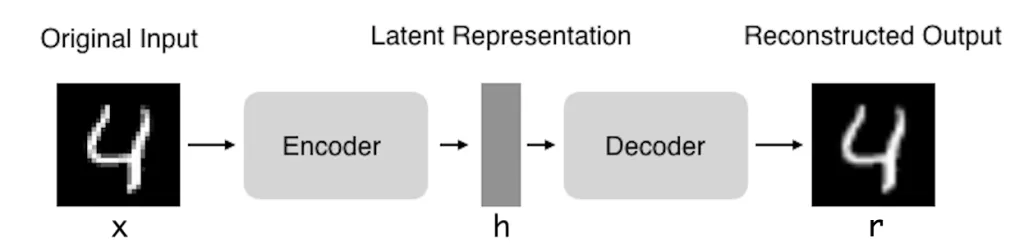
\includegraphics[width=\linewidth]{images/deep_learning/autoencoder.png}
\caption{Architecture of an Autoencoder. Source: \citep{autoencoder_architecture}}
\label{fig:autoencoder}
\end{figure}

\begin{enumerate}
\item \textbf{Encoder}: responsible for learning a useful representation of the input, also called as \textbf{embedding} or \textbf{latent representation} or even \textbf{code}. It can be formulated as an encoder function $h = f(x)$, where $x$ is the input and $h$ corresponds to the codification of the input in the latent space ($h: \mathbb{R}^D \rightarrow \mathbb{R}^K$, where $D$ and $K$ represent the dimensionality of the input and latent space, respectively).

\item \textbf{Decoder}: maps the learned latent representation $h$ back to the original input space ($\mathbb{R}^K \rightarrow \mathbb{R}^D$). It can be described as a reconstruction function $r = g(h)$, where $r$ is the reconstructed input.
\end{enumerate}

Since the exact copy of the input, $g(f(x)) = x$, is not especially useful, Autoencoders are intentionally designed to be unable to learn a perfect copy. Usually, Autoencoders are regularized in ways that allow them to learn an approximation of the identity function. By forcing the model to prioritize which input elements are relevant for reconstruction,  it often learns valuable properties of the data.

A typical Autoencoder architecture restricts the embedding dimensions ($h$) to be smaller than input $x$. Such Autoencoder is called \textbf{undercomplete}. By constraining $h$, the Autoencoder is forced to learn an undercomplete representation and must prioritize the most salient features of the input data during training. Moreover, the reconstructed input $r$ will not be a perfect copy of the input, and the undercomplete Autoencoders can be considered lossy compressors.

The learning process of Autoencoders involves the minimization of a loss function such as specified in \autoref{eq:loss-basic}:

\begin{equation}
\label{eq:loss-basic}
L(x, g(f(x)))
\end{equation}

\noindent
where $L$ is a loss function that computes the similarity between the reconstructed input $g(f(x))$ and the original input $x$. For instance, $L$ can be the \acf{mse} or the \acf{mae}

If the decoder is linear and $L$ is the \acs{mse}, the undercomplete Autoencoder will generate a subspace similar to \acs{pca}, described later in Section \ref{sec:pca} \citep{lecun2015deep}. On the other hand, Autoencoders with both nonlinear encoder and decoder can learn a more robust representation than \acs{pca}. However, if the encoder and decoder are too powerful, the Autoencoder can learn the identity function without extracting helpful information regarding the data distribution. For instance, each training sample $x^{(i)}$ can be expressed as the code $i$, and the decoder can learn to map these integer indices back to specific training examples. Nonetheless, this rarely occurs in practice \citep{lecun2015deep}.

Although the training of Autoencoders is similar to regular Neural Networks, some hyperparameters require special attention, such as:

\begin{itemize}
\item \textbf{Embedding size}: the size of the latent representation represents a tradeoff between compression and accurate reconstruction. A smaller size results in more compression, but the Autoencoder may be forced to drop relevant features for reconstruction. On the other hand, the higher the embedding size, the more likely it is that the Autoencoder will memorize or overfit the training data. Usually, this effect can be diminished by adding a term to the loss function that discourages memorization/overfitting (e.g., a regularizer).

\item \textbf{Number of Layers}: Vanilla Autoencoders are trained with a single hidden layer. However, training multilayer Autoencoders offers several advantages. First, depth can exponentially reduce the computational cost associated with representing a function. Furthermore, depth can also decrease the amount of training data required to train a useful Autoencoder \citep[p.~506]{goodfellow2016deep}, as the compact and expressive representations enable them to learn more robust and abstract features. Finally, experiments have shown that deep Autoencoders yield significantly better compression than equivalent shallow or linear Autoencoders \citep{hinton2006reducing}.

\item \textbf{Number of nodes per layer}: usually, Autoencoders have symmetric architecture. The number of nodes per layer in the encoder is the same as that in the decoder part, but inversely. In the case of undercomplete Autoencoders, as described earlier, the number of neurons per layer decreases at each layer and increases back in the decoder. In fact, symmetric architecture is not a mandatory rule but is commonly adopted in practice.

\item \textbf{Loss Function}: as discussed before, generally, the \acs{mse} and \acs{mae} are used to measure the differences between the original input and the consequent reconstruction. Similarly, binary cross-entropy may also be used for cases where the input is in the range [0-1]. However, other types of Autoencoders can apply different loss functions. For example, Sparse Autoencoders add a sparsity constraint (e.g., L1 regularization) as a penalty term, so only a fraction of the nodes will become active (i.e., nonzero values).
\end{itemize}

As pointed out by \cite{lecun2015deep}, the lower-dimensional representations of Autoencoders have some benefits, such as (i) they can improve the performance of tasks such as classification; (ii) fewer parameters require less memory and runtime; and (iii) the hints provided by the lower-dimensional space aid generalization.

\subsection{Representation Learning}

The success of an \acs{ml} system is closely tied to the choice and quality of data representation (commonly referred to as features) used for training. Although the criteria for valuable features depend on the task, it is widely acknowledged that there are sets of features that are representative of a dataset and can be applied to many downstream classifiers or predictors. Focusing on learning representations can yield significant benefits, especially in scenarios where a labeled dataset for a task is limited and using a larger unlabeled dataset is desirable to enhance the performance of the learning system.

\textit{Representation Learning} refers to the process of learning a parametric mapping from the raw input data domain into a feature vector or tensor that captures the underlying structure and patterns \citep{le2020contrastive}. This enables the extraction of more abstract and useful concepts that can improve the performance on multiple downstream tasks. Commonly, the input data have a high-dimensional space (e.g., images, text, or sound), and the goal is to encode these data into a meaningful lower-dimensional representation. Representation Learning ensures that the learned mapping generalizes well to new data samples, making it a powerful technique for improving performance on various tasks.

\cite{bengio2013representation} defines that a useful representation has the following properties: (i) local smoothness of input and representation; (ii) temporally and spatially coherent in a sequence of observations; (iii) multiple, hierarchically-organized explanatory factors which are shared across tasks; (iv) simple dependencies among factors; and (v) is sparsely activated for a specific input. In addition, especially for \acl{dl}, the authors in \citep{le2020contrastive} also define other core principles for suitable representation, which are:

\begin{itemize}
\item \textbf{Distribution}: expressive representation can be a proxy for an exponential amount of configuration for their size.

\item \textbf{Abstraction and Invariance}: helpful representations can capture more abstract concepts that are also invariant to local and small changes in the input data.

\item \textbf{Disentangled representation}: a well-designed representation should effectively capture the relevant factors of the data while retaining as much information as possible. At the same time, it is desirable to disentangle these factors, as this allows the reuse of learned features in other learning systems and may be beneficial for explainability. 
\end{itemize}

\acf{nlp} is probably one of the areas that most benefited from Representation Learning. With the advent of \acl{dl}, more useful representations have been obtained with embeddings computed from a large corpus of texts. In this case, the embeddings consist of a mapping from words represented as one-hot vectors into a distributed representation of real-valued numbers. Other commonly used words embedding methods include bag-of-words, skip-grams, and global vectors (GloVe) \citep{pennington2014glove, mikolov2013efficient}.

\subsection{Multitask Learning}

\acf{mtl} is a recent \acl{ml} technique in which multiple tasks are solved simultaneously, exploring common aspects and differences between them. This technique is inspired by the human learning process, in which the knowledge obtained in previous problems is applied to learn the pattern of a new problem \citep{zhang2017survey}. Through \acs{mtl}, the network can use relevant information in related tasks to improve generalization in all tasks. Besides, this technique can achieve comparable or even better performance than the corresponding single-task counterparts using much fewer training samples \citep{domhan2017using, singla2018multi}.

In a formal definition, given a set of $m$ learning tasks $\{T_i\}_{i=1}^m$, where all tasks or a subset of them are related to each other - but not identical -, the goal of \acs{mtl} is to help improve the learning process of a model for $T_i$ by using the knowledge included in the $m$ tasks. Moreover, there are two underlying factors for \acs{mtl} based on this definition. The first is task relatedness, which refers to understanding how distinct tasks are related. Such information can be applied to the design of \acs{mtl} models. Secondly, is the definition of the task itself. For example, there can be tasks of classification, regression, clustering, and many others. Consequently, different tasks result in particular \acs{mtl} settings.

Regarding the relatedness of \acs{mtl} tasks, three common issues must be addressed: what to share, when to share, and how to share. Starting with the ``when to share'' issue, the focus is choosing between single-task and multitasking problems. Generally, the decision is addressed by model selection techniques as cross-validation. The ``what to share'' defines the scheme of knowledge shared among all tasks. In this case, knowledge is usually shared in three forms: (i) feature-based, where joint features are learned among distinct tasks; (ii) instance-based, in which helpful data instances are identified and used for other tasks; and (iii) parameter-based, which uses model parameters (e.g., weights of \acl{dl} models) in a task to help learn model parameters in other tasks. Lastly, the ``how to share`` defines specific ways to share knowledge between tasks. For instance, in feature-based \acs{mtl}, the focus is on learning generic feature representations for multiple tasks that can be a subset or a transformation of source features. In parameter-based \acs{mtl}, there are four main approaches: task clustering, low rank, decomposition, and task relations. More details regarding each approach can be found in \citep{zhang2017survey}.

In terms of the nature of the tasks, \acl{mtl} can be divided into several categories \citep{zhang2018overview}, including:

\begin{itemize}
\item \textbf{Multitask supervised learning}: in this case, each task is a classification or regression problem. The goal is to predict labels for unseen data using a training dataset with labeled instances.

\item \textbf{Multitask unsupervised learning}: applied mainly for clustering problems, the goal is to identify functional patterns in a dataset of data instances only.

\item \textbf{Multitask semi-supervised learning}: similar to the supervised category, but each task in the training set contains labeled and unlabeled data.

\item \textbf{Multitask active learning}: each task exploits unlabeled data to help learn from labeled data (likewise the semi-supervised learning). However, distinctly unlabeled instances are selected to query their labels actively.

\item \textbf{Multitask reinforcement learning}: where the goal is to choose actions to maximize cumulative rewards for each task.

\item \textbf{Multitask online learning}: each task handles sequential data.

\item \textbf{Multitask multi-view learning}: aims to handle multi-view data with multiple sets of features to describe each instance.
\end{itemize}

From the \acl{ml} perspective, \acl{mtl} can be seen as a form of inductive transfer. The goal of inductive transfer is to take advantage of additional information sources to increase the performance of the current task learning. It helps a model by introducing an \textbf{inductive bias}. Therefore, a model can prefer some hypotheses over others. A typical example of inductive bias is L1 regularization, which leads a model toward sparse solutions. In the context of \acs{mtl}, the inductive bias is supplied by the auxiliary tasks. In this case, the model prefers the hypothesis that explains more than one task. According to \cite{Caruana1997}, the inductive transfer can decrease the learning process time and increase the generalization and intelligibility of the model. 

The inductive bias obtained through \acs{mtl} is intuitively compelling. In fact, the authors in \citep{ruder2017overview} cite a list of reasons why \acs{mtl} works. In the examples below, we consider that there are two related tasks $A$ and $B$ which rely on a shared representation $F$, as follows:

\begin{itemize}
\item \textbf{Implicit Data Augmentation}: \acl{mtl} offers a powerful approach to increasing the sample size for training a model. Since all tasks present specific noise patterns, the goal is to learn a helpful representation that generalizes well and is resilient to data-dependent noise. Consequently, a model trained on multiple tasks simultaneously can learn a more general representation. In contrast, training on a single task alone increases the risk of overfitting that specific task. By learning tasks $A$ and $B$ together, the model is able to obtain a more valuable representation $F$ by averaging the noise patterns.

\item \textbf{Attention Focusing}: When a task is characterized by a high degree of noise or the data is limited and high-dimensional, it can be challenging for a model to distinguish between relevant and irrelevant features. In this context, \acs{mtl} can aid by enabling the model to focus on genuinely significant features since other tasks will provide the additional evidence for feature importance.

\item \textbf{Eavesdropping}: some features $G$ may be relatively easy to learn for some task $B$, while being hard to learn for another task $A$. This may occur especially when (i) $A$ interacts with features in a complex way; or (ii) other features hamper the model's capability to learn feature $G$. Through the application of \acs{mtl} techniques, the model can learn $G$ through task $B$ (``eavesdrop''). As shown in \citep{abu1990learning}, it can be achieved by ``hints'', i.e., training the model directly to predict the most relevant features.

\item \textbf{Representation Bias}: \acs{mtl} biases the model in a way to build representations that are useful for multiple tasks. As stated by \cite{baxter2000model}, it aids a model to generalize better on new tasks in the future, as a hypothesis space that performs well for a significantly large number of training tasks will also perform well when learning new tasks as long as they are from the same environment.

\item \textbf{Regularization}: as discussed before, \acl{mtl} serves as a regularization technique by introducing an inductive bias to the model. This approach mitigates the risk of overfitting and decreases the Rademacher complexity of the model \citep{shalevshwartz2014understanding}, i.e., the capacity to fit random noise.
\end{itemize}

Compared to Transfer Learning, the setting of \acs{mtl} is similar but has some substantial differences. First, in \acs{mtl}, different tasks are treated equally, and the goal is to improve performance among all tasks. In contrast, Transfer Learning is focused on improving the performance of a specific target task with the help of one or more source tasks. In this case, the target task receives more emphasis than the source tasks. In other words, in \acs{mtl}, there is no distinction between different tasks, whereas, in Transfer Learning, the target tasks attract more attention. Second, from the perspective of knowledge flow, Transfer Learning transfers knowledge from the source task(s) to the target task. In contrast, \acl{mtl} knowledge sharing occurs between all pairs of tasks \citep{zhang2017survey}.

We can also compare \acs{mtl} with other methods to represent problems. For example, in Continual Learning \citep{chen2018lifelong}, the tasks are learned one by one sequentially, whereas, in \acs{mtl}, all tasks are learned together. Additionally, in multi-label problems, including multi-output regression, each data point is assigned to multiple categorical/numeric labels. In these cases, if each label is considered an individual task, they can be considered a particular case of \acl{mtl}, where different tasks always share the same data during the training and testing phases. Finally, in multi-view learning \citep{ZHAO201743}, a newer paradigm in \acl{ml}, each data point is represented with multiple views, each of which comes from a particular set of features. However, all the views are used together to learn the same task. Therefore, multi-view learning can be seen as single-task learning with multiple sets of features, which is, by definition, unlike \acs{mtl}.

\subsection{Network Explainability and Visualization}

For some time, \acl{dl} methods were considered black boxes because interpreting their outputs was difficult. To overcome this problem, some methods to visualize and explain the predictions of Neural Networks have been proposed in the specialized literature. Some of the most well-known methods are GradCam \citep{gradcam}, \acf{lime} \citep{lime}, DeepLIFT \citep{deeplift_old, deeplift_new}, and \acs{shap} \citep{shap2018}. 
 Furthermore, we cite other variations of \acs{shap} and highlight its advantages.

\subsubsection{SHAP}

The \acf{shap} is a method to explain the output of any machine learning model using a solid theoretical foundation of game theory. The classical Shapley values \citep{shapley1953value} from game theory and their related extensions are combined to optimal credit allocation with local explanations. Nowadays, the method is considered state-of-the-art for \acs{ml} explainability.

The Shapley values quantify each player's contribution to a game. In the context of \acl{ml}, the ``game'' is considered the model's outcome, while the ``players'' are represented by one or more features included in the model. In the case of images, specifically, pixels can be grouped (superpixels) to explain predictions distributed among them. Therefore, the goal of \acs{shap} is to measure the contribution of each feature concerning the model's prediction.

Given the original prediction model $f$ to be explained and the explanation model $g$, the Shapley value explanation is represented as an additive feature attribution method (\autoref{eq:shap_add}), which is a linear function of binary values:

\begin{equation}
\label{eq:shap_add}
g(z')=\phi_0+\sum_{j=1}^M\phi_jz_j'
\end{equation}

\noindent
where $z' \in \{0,1\}^M$ is the coalition (subset) vector, $M$ denotes the number of simplified input features (coalition size) and $\phi \in \mathbb{R}$ is the feature attribution for a feature $j$ (Shapley values). Many methods havve explanation models that matches the \autoref{eq:shap_add}, including \acs{lime} \citep{lime} and \textit{DeepLIFT} \citep{deeplift_old, deeplift_new}.

To compute the contribution of each feature ($\phi_i$), the \acs{shap} method requires the model to be retrained on all subsets of features $S \subseteq F$, where $F$ is the complete set of features. A corresponding importance value will be assigned to each feature to represent the effect on the model prediction when such feature is included. To compute this effect, a model is trained with the presence of that feature ($f_{S \cup \{i\}}$), and another model is trained without that feature ($f_S$). Subsequently, the predictions of the two models are compared for the current input $f_{S \cup \{i\}}(x_{S \cup \{i\}}) - f_S(x_S)$. In this case, $x_S$ denotes the values of the input features in the set $S$. The preceding differences are computed for all possible subsets since the effect of withholding a feature also depends on other features in the model. The Shapley values are the weighted average of all possible differences (\autoref{eq:shapley-values}):

\begin{equation}
\label{eq:shapley-values}
\phi_i = \sum_{S \subseteq F \setminus \{i\}} \frac{\left|S\right|!(\left|F\right| - \left|S\right| - 1)!}{\left|F\right|!}\left[f_{S \cup \{i\}}\right (x_{S \cup \{i\}}) - f_S(x_S)]
\end{equation}

Since a model is trained for every subset of $S$, the exact computation of Shapley values is expensive. For $\left|F\right|$ features, there is a total of $2^{\left|F\right|}$ subsets of S. However, in the paper that presents \acs{shap} \citep{shap2018}, the authors propose a model-agnostic approach to approximate Shapley values, called Kernel SHAP, and four other model-type-specific approximation methods: Linear SHAP, Low-Order SHAP, Max SHAP, and Deep SHAP. The Deep SHAP is a specific version of \acs{shap}, particularly designed for Deep Networks. The method is based on DeepLift \citep{deeplift_old, deeplift_new}, which approximates SHAP values by considering the input features independent of each other and the deep model as linear. In Deep SHAP, the SHAP values of the entire network are a combination of the SHAP values computed for smaller network components. It generates effective linearization from the SHAP values computed for each component. Please refer to the original paper for further explanation of other methods.

The SHAP method has the four properties of classical Shapley values:

\begin{enumerate}
\item \textbf{Efficiency:} the sum of the Shapley values for all players is equal to the value of the total coalition. 
\item \textbf{Symmetry}: all players have a fair chance to join the game.
\item \textbf{Dummy}: if a player $i$ has no contribution to a coalition $S$ (i.e., for each $S$, $f_{S \cup \{i\}} = f_S$), then its contributions is zero ($\phi_i = 0$).
\item \textbf{Additivity}: for any pair of games $a$ and $b$, $\phi(a + b) = \phi(a) + \phi(b)$. This property enables simple arithmetic summation.
\end{enumerate}

Some of the main advantages of \acs{shap} are discussed next. First, it is model-agnostic, i.e., \acs{shap} makes no prior assumption of the model and can work with any \acs{ml} algorithm. Second, this method ensures consistency. It means that even if features are removed from the data, the others continue to contribute with the same importance (Shapley values). Lastly, \acs{shap} can explain not only how each feature contributes to each sample (\textit{local interpretability}) but also at a global level (\textit{global interpretability}) by aggregating the local results.

\subsection{Dimensionality Reduction}

There are many applications for algorithms of dimensionality reduction. Usually, these methods are used when the cardinality of features is significantly larger than the number of samples (also called the ``\textit{curse of dimensionality}''). However, they may also be applied to project data into a lower-dimensional space (usually 2D/3D), aiming to simplify the visualization and search for patterns in data. The following subsections describe two methods of dimensionality reduction used in this work.

\subsubsection{Principal Component Analysis}
\label{sec:pca}

The \acf{pca} \citep{pca} is an unsupervised \acl{ml} algorithm for dimensionality reduction with minimal information loss. In \acs{pca}, the information is based on data variance. The idea is that features with a high variance contain more information because their data are more distributed than features with a low variance. Accordingly, \acs{pca} projects the data into a subspace where the axis with the highest variances, also called \textit{principal components}, are preserved. More details of \acs{pca} are described below.

The foremost step of \acs{pca} is to compute the \textbf{eigenvectors} (principal components) of the input data. The eigenvectors explain the variance of the data along the new axes and determine the direction in the new feature space. In \acs{pca}, the eigenvectors are organized into a projection matrix and each eigenvector is associated with an \textbf{eigenvalue}. The eigenvalue can be interpreted as the magnitude of the corresponding eigenvector. If the eigenvalues have a similar magnitude, it can be considered a valuable indicator that the original data are already in a suitable subspace. Otherwise, if the magnitude of some eigenvalues is much higher than others, the corresponding eigenvectors may be chosen since they contain more information about our data distribution. Likewise, eigenvalues near zero are less informative and may be discarded when constructing the new subspace. 

The classical approach of \acs{pca} \citep{pca} computes the covariance matrix, where each element represents the covariance between two features, as computed by \autoref{eq:covariance}:

\begin{equation}
\label{eq:covariance}
\sigma_{jk} = \frac{1}{n-1}\sum_{i=1}^{n}(x_{ij} - \bar{x_j})(x_{ik} - \bar{x}_k)
\end{equation}

\noindent
which can be rewritten in matrix form as \autoref{eq:covariance2}:

\begin{equation}
\label{eq:covariance2}
S = \frac{1}{n-1}((x - \bar{x})^T(x - \bar{x}))
\end{equation}

\noindent
where $\bar{x}$ is a D-dimensional vector, in which each value corresponds to the average of each feature, and $n$ is the number of features per sample. In addition, $x$ is the data matrix, where a row represents each sample and the features are columns. In practice, if we have a dataset with four features, for instance, the covariance matrix will have the following structure:

$$
\begin{bmatrix}var(1) & cov(1,2) & cov(1,3) & cov(1,4) 
\\ cov(1,2) & var(2) & cov(2,3) & cov(2,4)
\\ cov(1,3) & cov(2,3) & var(3) & cov(3,4)
\\ cov(1,4) & cov(2,4) & cov(3,4) & var(4)
\end{bmatrix}
$$

\noindent
where the main diagonal corresponds to the variance of each dimension and the remaining elements are the covariance between each dimension pair. An attractive property of the covariance matrix is that the sum of the main diagonal is always equal to the sum of eigenvalues.

The eigenvectors and eigenvalues of \acs{pca} can also be computed using the correlation matrix. Although the resulting matrices are different, they result in the same eigenvectors and eigenvalues since the correlation matrix is given by the standardization of the covariance matrix (\autoref{eq:correlation}):

\begin{equation}
\label{eq:correlation}
corr(x,y) = \frac{cov(x,y)}{\sigma_x \sigma_y}
\end{equation}

Given the projection matrix $W$ computed by \acs{pca}, the original data $x$ can be projected onto the new subspace $S$ by applying \autoref{eq:pca_transform}:

\begin{equation}
\label{eq:pca_transform}
S = (x-\bar{x}) \times W
\end{equation}

Note that the original space $x$ can be reconstructed by applying \autoref{eq:pca_inverse}:

\begin{equation}
\label{eq:pca_inverse}
x = (S \times W^{-1}) + \bar{x}
\end{equation}

Finally, the \acf{lda} \citep{izenman2013linear} is a similar dimensionality reduction technique. In contrast to \acs{pca}, \acs{lda} is a supervised method that maximizes component axes for class separation. Although it appears that \acs{lda} performs better than \acs{pca} in reducing dimensionality for classification problems, this is not always true. Performance comparisons in terms of accuracy for image recognition problems have shown that \acs{pca} performs better than \acs{lda} if the number of samples per class is relatively low \citep{martinez2001pca}.

\subsubsection{t-SNE}

The \acf{tsne}, developed by \cite{tsne}, is a nonlinear dimensionality reduction method well suited for visualizing high-dimensional datasets. It is based on Stochastic Neighbor Embedding \citep{sne}, but the main difference is the utilization of the \textit{t}-Student distribution to represent the data in low dimensions.

The \acs{tsne} algorithm comprises two main stages. First, the symmetric probability of points in the original high-dimensional space is computed. Higher probabilities are assigned to similar points, whereas dissimilar points are assigned a lower probability. Such probabilities are computed using a \textit{t}-Student kernel with a given degree of freedom. Secondly, a similar probability distribution is defined over the points mapped into the low-dimensional space. The Kullback-Leibler divergence (also called relative entropy) between these two distributions is minimized through a gradient descent technique. A simplified version of \acs{tsne} is shown in Algorithm \ref{alg:tsne}, and the details are explained below.

\begin{algorithm}[ht]
\caption{Simple version of t-Distributed Stochastic Neighbor Embedding}
\label{alg:tsne}
\begin{algorithmic}
    \State \textbf{Data:} data set $X = \{x_1, x_2, ..., x_n\}$,
    \State cost function parameter: perplexity $\rho$,
    \State optimization parameters: number of iteration $T$, learning rate $\eta$, momentum $\alpha(t)$.
    \State \textbf{Result:} low-dimensional data representation $\gamma^{(T)} = \{y_1, y_2, ..., y_n\}$.
    \Begin 
        \State compute pairwise affinities $p_{j|i}$ with perplexity $\rho$ (using \autoref{eq:tsne_pij})
        \State set $p_{ij} = \frac{p_{j|i} + p_{i|j}}{2n}$
        \State sample initial solution $\gamma^{(0)} = \{y_1, y_2, ..., y_n\}$ from $\mathcal{N}(0, 10^{-4}I)$
        \For{i=1}{T}
        \Begin
            \State compute low-dimensional affinities $q_{ij}$ (using \autoref{eq:tsne_qij})
            \State compute gradient $\frac{\partial C}{\partial \gamma}$ (using \autoref{eq:tsne_grad})
            \State set $\gamma^{(t)} = \gamma^{(t-1)} + \eta \frac{\partial C}{\partial \gamma} + \alpha(t)(\gamma^{(t-1)} - \gamma^{(t-2)})$
        \End
    \End
\end{algorithmic}
\end{algorithm}

Given an object $i$, and each potential neighbor $j$ in the high-dimensional space, the joint probability $p_{ij}$ that computes the pairwise similarity between $i$ and $j$ is defined as in \autoref{eq:tsne_pij}:

\begin{equation}
\label{eq:tsne_pij}
p_{ij} = \frac{exp(-d_{ij}^2)}{\sum_{k \neq i}exp(-d_{ik}^2)}
\end{equation}

In the original SNE, a conditional probability $p_{i|j}$ is used instead. Also, the t-SNE employs the scaled Euclidean Distance as the dissimilarity metric $d_{ij}^2$ between two high-dimensional points $x_i$ and $x_j$ (\autoref{eq:tsne_dij}). However, other distance metrics can also be used when appropriate. One important detail is that the pairwise similarity $p_{ij}$ is not robust to outliers since $\left\| x_i - x_j\right\|^2$ will be large. In these cases, the values of $p_{ij}$ will be minimal and the location of its low-dimensional map point will have minimal effect on the cost function. In practice, such problem is prevented by computing $p_{ij} = \frac{p_{j|i} + p_{i|j}}{2n}$ instead. This ensures that $\sum_j p_{ij} > \frac{1}{2n}$ for all the data points $x_i$. As a result, each data point $x_i$ has a significantly higher contribution to the cost function.

\begin{equation}
\label{eq:tsne_dij}
d_{ij}^2 = \frac{\left\| x_i - x_j \right\|^2}{2\sigma_i^2}
\end{equation}

\noindent
where $\sigma_i$ can be either defined by experimentation or via a binary search that makes the entropy of the distribution over neighbors equal to $log\ \rho$. In this case, $\rho$ is an input parameter of the cost function called ``perplexity.'' The perplexity may be interpreted as a measure of the effective number of neighbors and is defined by \autoref{eq:tsne_perp}:

\begin{equation}
\label{eq:tsne_perp}
\rho(P_i) = 2^{H(P_i)}
\end{equation}

\noindent
where $H(P_i)$ is the Shannon entropy of probability $P_i$ measured in bits by \autoref{eq:tsne_entropy}:

\begin{equation}
\label{eq:tsne_entropy}
H(P_i) = -\sum_j p_{j|i}\ log_2\ p_{j|i}
\end{equation}

In general, the performance of t-SNE is reasonably robust to changes in perplexity and typical values are between 5 and 50.

The similarity in low-dimensional space is given by \autoref{eq:tsne_qij}:

\begin{equation}
\label{eq:tsne_qij}
q_{ij} = \frac{exp(-\left\| y_i - y_j \right\|^2)}{\sum_{k \neq i} exp(-\left\| y_i - y_k \right\|^2)}
\end{equation}

\noindent
where $y_i$ and $y_j$ represent the low-dimensional counterparts of the
high-dimensional data points $x_i$ and $x_j$. Usually, for tasks in which the dimensionality of the data is reduced to 2D or 3D, the \textit{t}-Student distribution is applied with one degree of freedom, and \autoref{eq:tsne_qij} can be rewritten as \autoref{eq:tsne_qij_1}

\begin{equation}
\label{eq:tsne_qij_1}
q_{ij} = \frac{(1 +\left\| y_i - y_j \right\|^2)^{-1}}{\sum_{k \neq l} (1 +\left\| y_k - y_l \right\|^2)^{-1}}
\end{equation}

Finally, \acs{tsne} attempts to minimize a single Kullback-Leibler divergence (\autoref{eq:tsne_cost}) between a joint probability distribution $P$ in the high-dimensional space and a joint probability distribution $Q$ in the low-dimensional space:

\begin{equation}
\label{eq:tsne_cost}
C = KL(P||Q) = \sum_i\sum_j p_{ij} log \frac{p_{ij}}{q_{ij}}
\end{equation}

In contrast to the SNE implementation, the \acs{tsne} is symmetric since $p_{ij} = p_{ji}$ and $q_{ij} = q_{ji}$ $\forall i,j$. The main advantage of such symmetry is the simpler gradient expression, which is faster to compute. The gradient of cost function $C$ with respect to point $y_i$ is given by \autoref{eq:tsne_grad}:

\begin{equation}
\label{eq:tsne_grad}
\frac{\partial C}{\partial y_i} = 4 \sum_j (p_{ij} - q_{ij})(y_i - y_j)
\end{equation}

And the set $\gamma^{(t)} = \{y_1, y_2, ..., y_N\}$ is updated by the momentum term given by \autoref{eq:tsne_update}:

\begin{equation}
\label{eq:tsne_update}
\gamma^{(t)} = \gamma^{(t-1)} + \eta\frac{\partial C}{\partial \gamma} + \alpha(t)(\gamma^{(t-1)} - \gamma^{(t-2)})
\end{equation}

\noindent
where $\gamma^{(t)}$ indicates the solution at iteration $t$, $\eta$ denotes the learning rate, and $\alpha(t)$ represents the momentum at iteration $t$. For the derivation of \acs{tsne} gradient, please refer to Appendix A of \citep{tsne}. 

Compared with \acs{pca}, the \acs{tsne} does not conserve the original space's distances or densities. Only the neighborhood is preserved, but up to a certain degree. Furthermore, due to the non-deterministic behaviour of \acs{tsne}, there is no guarantee of convergence to the global optimum of the cost function and the performance is not clearly defined for general dimensionality reduction tasks.  

\subsection{Performance Measures} \label{sec:measures}

There are a variety of performance measures to evaluate algorithms in binary classification problems. In common, most of these metrics take into account some of/all the four possible results present in the binary confusion matrix: \acfp{tp}, \acfp{tn}, \acfp{fp}, and \acfp{fn}. In this subsection, the evaluation metrics used in this study are described. Comments on the advantages and disadvantages of each are also made when appropriate. 

\subsubsection{Accuracy}

Accuracy is one of the most commonly used metrics to evaluate binary classifiers. In simple terms, it measures how many predictions were correct among all samples in a given dataset. The output of this metric is a score $\in [0, 1]$, which is interpreted as the proportion of correct predictions (i.e., true positives and true negatives) among the total number of samples analyzed. Accuracy is described by \autoref{eq:accuracy}:

\begin{equation}
\label{eq:accuracy}
Accuracy = \frac{TP + TN}{TP + TN + FP + FN}
\end{equation}

Although accuracy is one of the most used metrics to evaluate binary classifiers, it is not well suited for unbalanced datasets. Suppose a dataset in which 80\% of the samples are from the positive class, and the remaining are from the negative class. If some classifier outputs only the positive class, the overall accuracy will be 80\%. Therefore, accuracy must only be considered valid when the class distributions are considerably uniform.

\subsubsection{Precision \& Recall} \label{precision-recall}

Precision and Recall are two metrics highly adopted in the evaluation of binary classifiers. While Precision measures how much we can trust a model when it predicts the positive class, Recall measures how accurate a model is regarding the positive class. In other words, the Precision metric answers the question ``\textit{given the positive predictions, how many were correct?}'', while Recall answers ``\textit{given the positive samples, how many predictions were correct?}''. Precision and Recall are also known as \acf{ppv} and Sensitivity, respectively, and are defined by Equations \ref{eq:precision} and \ref{eq:recall}: 

\begin{equation}
\label{eq:precision}
Precision = \frac{TP}{TP + FP}
\end{equation}

\begin{equation}
\label{eq:recall}
Recall = \frac{TP}{TP + FN}
\end{equation}

Even though the Precision and Recall metrics are considered more robust than accuracy for evaluating binary classifiers, both metrics present some drawbacks. First, they are purpose-specific. For example, Precision is a better choice when we want to trust the prediction of the positive class. However, if a model is optimized to maximize Precision only, it can bias the classifier to avoid uncertain positive samples, thereby increasing the number of false negatives. On the other hand, Recall is more pertinent when we need a classifier that may correctly identify positive samples, although it can generate more false positives. Hence, in the case of a problem where Precision and Recall are equally important, the f-measure can be computed to generate a balanced score between these two metrics. The f-measure is better described in the following subsection.

Secondly, by taking a closer look at the Equations \ref{eq:precision} and \ref{eq:recall}, we can notice that they do not consider the True Negatives. Therefore, both metrics are more appropriate when the positive class is more important than the negative class. This is the case for detection problems, for example, where identifying the negative class (usually background) is less important than the positive class (object of interest). Nevertheless, this is not always true for some classification problems. For instance, in fraud-detection problems, the correct prediction of the True Negatives has a higher priority over the True Positives. For these cases, we can compute the \acl{npv} and Specificity metrics, which will be described later.

\subsubsection{F-measure}

The f-measure, also called f-score or f1-score, is a metric that balances the values of Precision and Recall. The importance of f-measure is better understood by an example. Suppose there is a face detection problem where two different models, named $A$ and $B$, are applied to an image with ten faces. Model A returned five detections, where 3 were real faces (\acs{tp}), and 2 were incorrect. In this case, model A has a 30\% Recall (3 out of 10 detected faces) and 60\% Precision (3 out of 5 correct predictions). Otherwise, model B returned two detections, which were all real faces. In this case, the Recall is 20\% (2 out of 10 detected faces), and the Precision is 100\% (all detections were real faces). Therefore, if Precision and Recall are equally crucial for this problem, which model is better: model $A$ with 30\% of Recall and 60\% of Precision, or model $B$ with 20\% of Recall and 100\% of Precision? To answer this problem, we can compute the f-measure described by \autoref{eq:f-measure}: 

\begin{equation}
\label{eq:f-measure}
F1 = 2\frac{Precision \cdot Recall}{Precision + Recall}
\end{equation}

In the example cited above, the f-measure of model $A$ is 40\%, while the model $B$ is 33.3\%. Therefore, model $A$ can be considered a better model for this case because it has a higher f-measure and, consequently, a better equilibrium between Precision and Recall.

By definition, the f-measure is considered the harmonic mean between Precision and Recall. This is harmonic because, in contrast to the arithmetic mean, the metric cannot be made arbitrarily large by changing only the Precision or Recall to a larger value (while keeping the other metrics unchanged). Therefore, to increase f-measure considerably, both Precision and Recall must be higher simultaneously.

\subsubsection{F-Beta}

F-Beta is a generalization of F-measure. It adds a $\beta$ term to weigh how much Recall is more important than Precision. The F-Beta is defined by \autoref{eq:f-beta}:

\begin{equation}
\label{eq:f-beta}
F_\beta = \frac{(1 + \beta^2) \cdot P \cdot R}{\beta^2 \cdot P + R}
\end{equation}

As can be noticed, when $\beta=1$, the original formula of f1-score is obtained. Another typical value is $\beta=2$, generating the f2-score. In this case, the Recall has a higher weight than Precision. In other words, better Recall is more critical for the classifier than Precision. This is useful to ensure that the classifier is better at identifying the positive class, even though it might generate more false positives. In the detection example cited before, the detector would try to detect as many real faces as possible but would return more false positives (detections that are not real faces).

\subsubsection{Negative Predictive Value \& Specificity}

The metrics Specificity and \acf{npv} are equivalent to Recall and Precision, respectively, but for the negative class. In analogy to Precision and Recall, the Specificity answers the question ``\textit{given the negative samples, how many predictions were correct?}'', while the \acs{npv} answers ``\textit{given the negative predictions, how many were correct?}''. These metrics are defined by Equations \ref{eq:specificity} and \ref{eq:npv}:

\begin{equation}
\label{eq:specificity}
Specificity = \frac{TN}{TN + FP}
\end{equation}

\begin{equation}
\label{eq:npv}
NPV = \frac{TN}{TN + FN}
\end{equation}

Since both \acs{npv} and Specificity are similar to Precision and Recall, they share the same problems of these metrics described in Section \ref{precision-recall}. Hence, \acs{npv} and Specificity are purpose-specific (but for the negative class) and, analogously, do not consider the positive class.

\subsubsection{\acl{mcc}} \label{sec:mcc}

The \acf{mcc}, also known as the phi ($\phi$) coefficient, is a binary classification metric that considers all four categories: \aclp{tp}, \aclp{tn}, \aclp{fp}, and \aclp{fn}. It was introduced by biochemist Brian W. Matthews in 1975 \citep{matthews1975comparison} and is defined by the \autoref{eq:mcc}

\begin{equation}
\label{eq:mcc}
MCC = \frac{TP \times TN - FP \times FN}{\sqrt{(TP + FP)(TP + FN)(TN + FP)(TN + FN)}}
\end{equation}

The \acs{mcc} is considered a balanced metric and can be used even in highly unbalanced datasets. The output of \acs{mcc} is a normalized coefficient between $-1$ and $+1$. A coefficient of $+1$ indicates a perfect prediction, whereas $-1$ represents the total disagreement between the prediction and ground truth. In addition, a coefficient of $0$ indicates that the predictions are not better than random guesses. 

Because \acs{mcc} considers the four possible results of binary classification problems, it presents some advantages compared to other classification metrics. For example, suppose a trained classifier with a confusion matrix of TP = 90, \acs{fp} = 5, TN = 1, and FN = 4. In this case, the accuracy is 91\% and the f-measure is 95.24\%. On the other hand, the \acs{mcc} gives a score of 0.14, which means the algorithm is mainly predicting the most frequent class and performing similarly to random guessing. As suggested by \cite{chicco2017ten}, the use of \acs{mcc} is highly encouraged to evaluate performance in the test set of any binary classification problem.

\subsubsection{Equal Error Rate}

The performance of biometric systems is usually measured using metrics such as \acf{far}, \acf{frr}, and \acf{eer}. The \acl{far}, also known as \acf{fmr}, is the probability of an incorrect match between a given input pattern and a non-matching template. In other words, it computes the proportion of invalid inputs that are incorrectly accepted. On the other hand, the False Rejection Rate, also known as \acf{fnmr}, represents the likelihood of a system falsely rejecting a match between the input pattern and a genuine matching template. Alternatively, it computes the proportion of valid matches incorrectly rejected. According to \cite{ross2006handbook}, \acs{far} and \acs{frr} can be formally defined in the continuous case by the Equations \ref{eq:far} and \ref{eq:frr}, respectively:

\begin{equation}
\label{eq:far}
FAR(\tau) = \int_{\tau}^{\infty} p(s|impostor)\ ds
\end{equation}

\begin{equation}
\label{eq:frr}
FRR(\tau) = \int_{\tau}^{\infty} p(s|genuine)\ ds
\end{equation}

\noindent
where $p(s|impostor)$ and $p(s|genuine)$ correspond to the probability distributions of a score $s$ under genuine and impostor conditions, appropriately, and $\tau$ is a threshold for defining whether a given individual is genuine or an impostor.

Finally, the \acs{eer} is designated by the point at which the \acs{far} and \acs{frr} curves intercept each other (see \autoref{fig:eer}). Therefore, \acs{eer} represents the rate at which both acceptance and rejection errors are equal, i.e., $FAR = FRR$ or $p(s|impostor) = p(s|genuine)$. All the mentioned metrics (\acs{far}, \acs{frr}, and \acs{eer}) are inversely proportional to the performance of the biometric system (the lower, the better).

\begin{figure}[h]
\centering
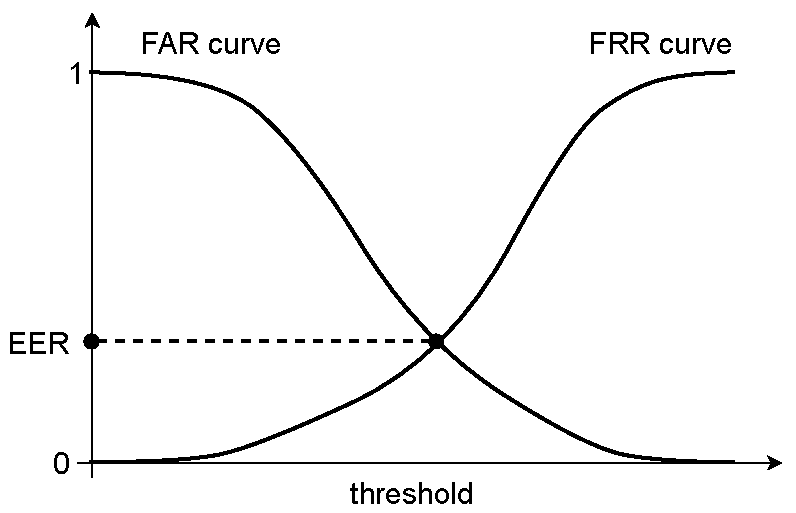
\includegraphics[height=2.1in]{images/metrics/EER.pdf}
\caption{The typical curves of the \acs{far} and \acs{frr} error rates, plotted side by side, in relation to the threshold $\tau$ configured for the system. The \acs{eer} is represented by the intersection point of the curves. Source: own elaboration.}
\label{fig:eer}
\end{figure}

Since \acs{far} and \acs{frr} are computed for a given threshold $\tau$, biometric systems can be calibrated by manually choosing the threshold that best fits the desired needs. However, this represents a tradeoff between convenience and security. For example, when security issues are critical (e.g., banking systems), threshold $\tau$ may be adjusted in a way that the \acs{far} is minimal. However, genuine users may have blocked access until the system is entirely sure about their profile. On the other side, if $\tau$ is fine-tuned to improve user convenience, the system can allow access to non-legitimate users.

\subsubsection{Wing Loss} \label{sec:wingloss}

Wing loss is a recently proposed function specially designed for facial landmark localization. It was introduced as an alternative to the commonly used \acs{mse} and \acs{mae} losses. The function is named after its shape, which resembles a wing (see \autoref{fig:wing_loss}). It was created by \citep{wingloss} and can be defined by \autoref{eq:wingloss}: 

\begin{equation}
\label{eq:wingloss}
wing(x) = \begin{cases}
w\ln(1 + \left | x \right | / \epsilon) & if\ \left | x \right | < w\\ 
\left | x \right | - C & otherwise 
\end{cases}
\end{equation}

\noindent
where $w$ is a non-negative constant that defines the range of the nonlinear part to $(-w, w)$, $\epsilon$ limits the curvature of the nonlinear region, and $C = w - w\ln(1 + w / \epsilon)$ is another constant that smoothly links the piecewise-defined linear and nonlinear parts. A critical detail regarding Wing Loss is that $\epsilon$ may not be set to a very small value because it makes the training unstable and causes an explosion of gradients.

\begin{figure}[htb]
\centering
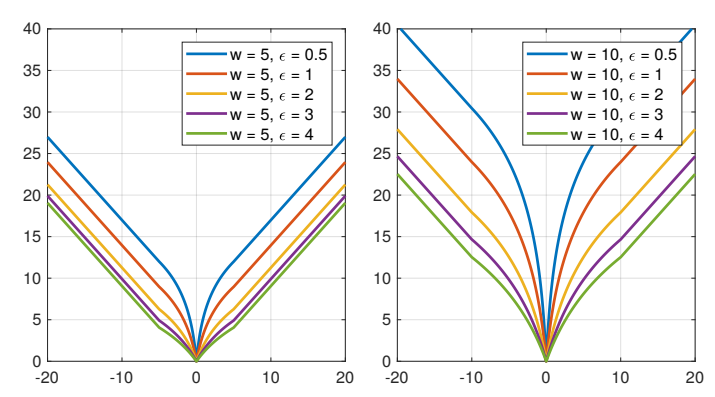
\includegraphics[width=0.8\linewidth]{images/metrics/wing_loss.png}
\caption{Wing loss function (\autoref{eq:wingloss}) plotted for different settings of $w$ and $\epsilon$. Source: \citep{wingloss}.}.
\label{fig:wing_loss}
\end{figure}

The main characteristic of Wing loss is that it amplifies the impact of samples with small and medium-range errors during the training step. The influence of small errors is enhanced by the $\ln$ component in the formula. In addition, in the case of large errors, Wing loss promotes a fast recovery behaving as L1 and being robust to outliers.

\subsection{The \icao Standard}

In 1980, the \acf{icao} began a project focused on the standardization of automatic biometric identification of people using machines \citep{icao2003report}. A specific working group was established to determine the most suitable way of ``uniquely encoding a particular physical characteristic of a person into a biometric-identifier that can be machine-verified to confirm the presenter's identity'' \citep{icao2003report}. Initially, three physical attributes were chosen for possible applications: face, fingerprint, and iris. Later, in the ``Berlin resolution'' (2002), the ICAO has chosen the face as the primary globally interoperable biometric trait for machine-assisted identity confirmation in \acf{mrtd} \citep{ferrara2012face}. However, the decision also states the possibility of identity confirmation through a fingerprint or iris to support machine-assisted decisions.

Following the ICAO guidelines, the \acf{iso}, together with the \acf{iec}, proposed a standard for facial photography to be used in electronic passports. The \icao \citep{iso-iec} standard specifies rules and a record format for encoding, recording, and transmitting facial image information. It also defines a set of environmental conditions, photographic properties, shooting features, and digital attributes of facial images. For example, a facial image may have a uniform background with the absence of shadows in any region of the image to be included in an electronic passport. The complete list of requirements can be seen in \autoref{tab:icao}, and examples of non-compliant images for each requirement are given in \autoref{fig:icao}. The \icao standard is also referenced in the ANSI/NIST-ITL 1–2011 standard \citep{nist2011} as one of the standard profiles for face acquisition. In 2019, a new version of the \icao standard was released. The \icaonew provides more detailed information about each requirement evaluation.

\begin{table}[tb]
% \scriptsize
\footnotesize
% \small
\centering
\caption{Description of facial image quality tests performed by \biolab, according to \icao standard.}
\label{tab:icao}
\begin{tabular}{|c|c|}
\hline
\rowcolor[HTML]{9B9B9B} 
\textbf{Req. \#} & \textbf{Test description} \\ \hline
\rowcolor[HTML]{C0C0C0} 
\multicolumn{2}{|c|}{\cellcolor[HTML]{C0C0C0}\textbf{Facial feature extraction tests}} \\ \hline
1 & Eye center location accuracy \\ \hline
2 & Face location accuracy \\ \hline
\rowcolor[HTML]{C0C0C0} 
\multicolumn{2}{|c|}{\cellcolor[HTML]{C0C0C0}\textbf{Geometric tests}} \\ \hline
3 & Eyes distance (min. 90 pixels) \\ \hline
4 & Relative vertical position \\ \hline
5 & Relative horizontal position \\ \hline
6 & Ratio of head width \\ \hline
7 & Ratio of head height \\ \hline
\rowcolor[HTML]{C0C0C0} 
\multicolumn{2}{|c|}{\cellcolor[HTML]{C0C0C0}\textbf{Photographic and pose-specific tests}} \\ \hline
8 & Blurred \\ \hline
9 & Looking away \\ \hline
10 & Ink marked/creased \\ \hline
11 & Unnatural skin tone \\ \hline
12 & Too dark/light \\ \hline
13 & Washed out \\ \hline
14 & Pixelation \\ \hline
15 & Hair across eyes \\ \hline
16 & Eyes closed \\ \hline
17 & Varied Background \\ \hline
18 & Roll/pitch/yaw rotations greater than a predefined thresholds \\ \hline
19 & Flash reflection on skin \\ \hline
20 & Red eyes \\ \hline
21 & Shadows behind head \\ \hline
22 & Shadows across face \\ \hline
23 & Dark tinted lenses \\ \hline
24 & Flash reflection on lenses \\ \hline
25 & Frames too heavy \\ \hline
26 & Frame covering eyes \\ \hline
27 & Hat/cap \\ \hline
28 & Veil over face \\ \hline
29 & Mouth open \\ \hline
30 & Presence of other faces or toys too close to face \\ \hline
\end{tabular}
\end{table}

\begin{figure}[h]
\centering
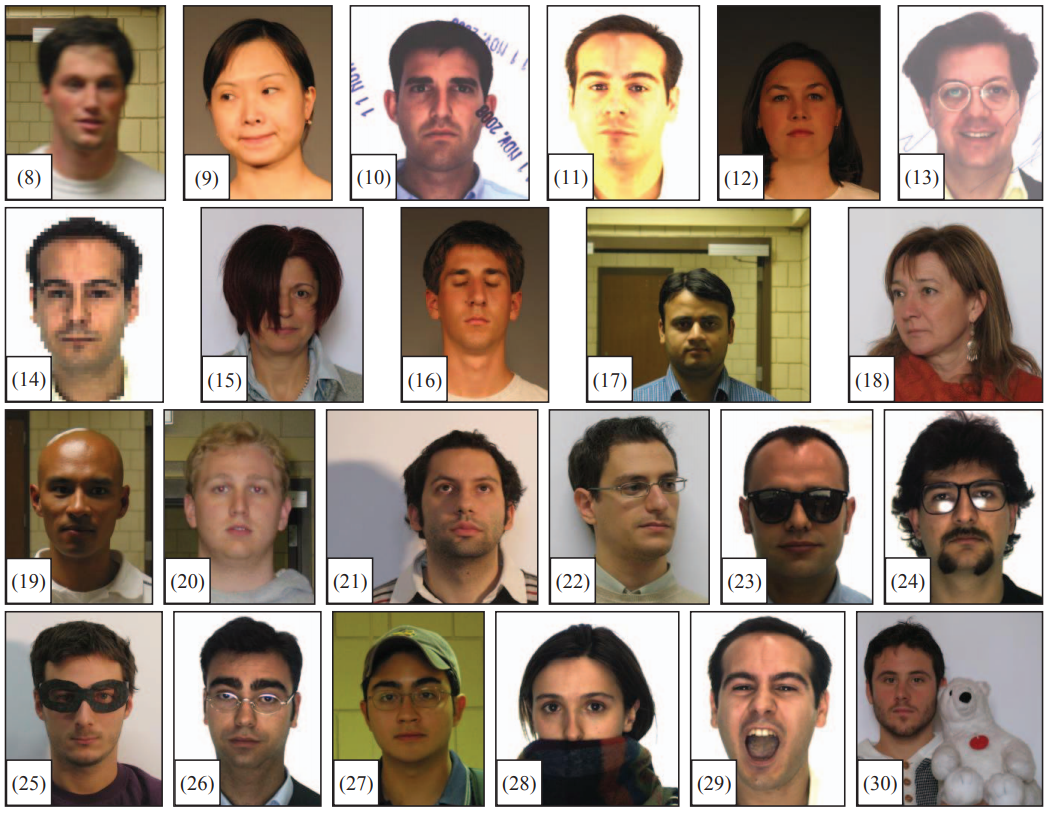
\includegraphics[width=\linewidth]{images/dataset/icao.png}
\caption{Examples of non-compliant images for the requirements 8-30 listed in Table \ref{tab:icao}. Source: \cite{maltoni2009biolab}.}
\label{fig:icao}
\end{figure}

\subsection{\fvcongoing} \label{sec:fvcongoing}

The \acf{fvc} is an event organized by four leading institutions: \textit{Biometric System Laboratory} (University of Bologna), \textit{Pattern Recognition and Image Processing Laboratory} (Michigan State University), \textit{Biometric Test Center} (San Jose State University), and \textit{Biometric Recognition Group - ATVS} (Universidad Autonoma de Madrid). The main goal of the \acs{fvc} was to benchmark systems that evaluate fingerprint images. Initially, the competitions used to happen biannually (2000, 2002, 2004, and 2006), and such events drew attention from the academic community and the industry related to biometrics. Over the years, the \acs{fvc} has become a reference for evaluating fingerprint systems, allowing research groups, private companies, and even individual developers to compare their methods and follow state-of-the-art fingerprint research.

After 2006, the organizers of \acs{fvc} decided to create the \fvcongoing. It turned the original biannual \acs{fvc} into an ongoing competition, i.e., every participant could register and submit new algorithms continuously. Moreover, new competitions regarding fingerprints were added to \fvcongoing, like fingerprint orientation extraction, fingerprint indexing, and minutiae matching.

In 2012, a new benchmark category related to the \icao standard was added to \fvcongoing \citep{ferrara2012face}, called \acf{ficv}. The main goal of this benchmark is to evaluate algorithms that assess the compliance of face images with the ISO standard. In total, 24 out of 30 requirements are evaluated by the \acs{ficv}: the \eyecenterlocation and all photographic and pose-specific tests (8--30) - see \autoref{tab:icao}. Moreover, the \acs{ficv} evaluates whether the image can be converted to a Token Format (see Section 9.2.3 in \citep{iso-iec}) based on the eye positions predicted by a submitted algorithm. In short, an image is considered \textit{tokenizable} (without padding) if:

\begin{itemize}
\item the distance ($E_{Dist}$) between eyes is at least 60 pixels;
\item the rectangular region of size $W \times H$ (with $W=4\cdot E_{Dist}$ and $H=W \cdot 4/3$), determined so that the eyes are horizontally aligned and their center is in position $C_E=(W\cdot1/2,W\cdot3/5)$, is totally enclosed in the original image (see \autoref{fig:icao_token}).
\end{itemize}

\begin{figure}[h]
    \centering
    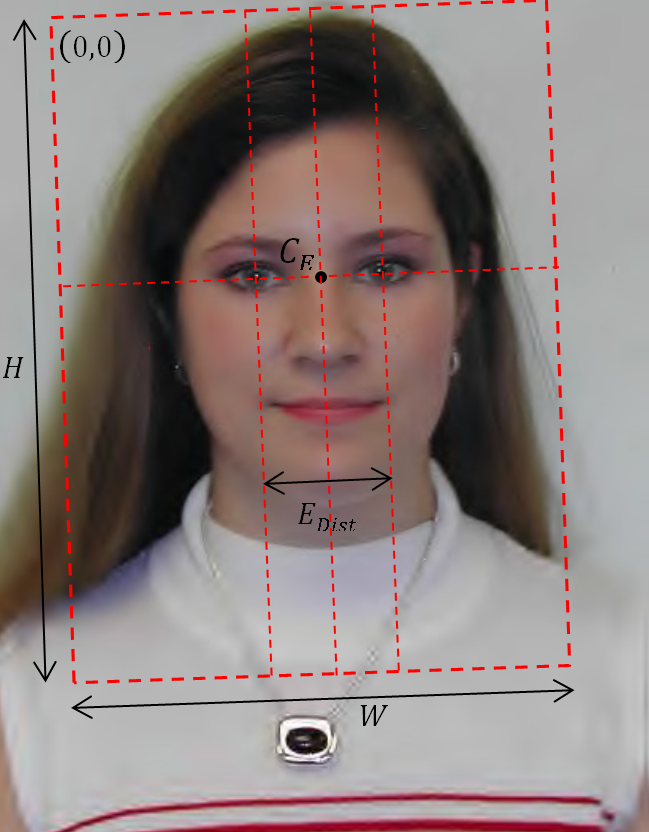
\includegraphics[height=3.0in]{images/dataset/icao_tokenizable.png}
    \caption{Geometric characteristics of the token image format. Source: \citep{fvcongoing}.}
    \label{fig:icao_token}
\end{figure}

Two datasets are used to benchmark the algorithms submitted to the \acs{ficv} competition: \ficvtest and \ficvofficial. The \ficvtest is a small but representative dataset (720 images) that is only used to test the compliance of the submitted algorithm with the testing protocol (described below). The results computed on this dataset are only visible to the participant and are not considered as official results of the competition. On the other hand, the \ficvofficial contains 4868 images and is private to all participants. Such dataset is detailed in \cite{ferrara2012face}. All results presented in the literature and this thesis were computed using the \ficvofficial dataset.

All the participants who wish to submit an algorithm for evaluation in the \acs{ficv} competition must follow a well-defined protocol. The algorithm must be submitted as a Windows 32 bits (Win32) console application as an executable file of up to 50MB compressed using the zip format. Such executable receives a face image as input and must output the coordinates $(x, y)$ of the left and right eye centers and a score in the range of $[0, 100]$ to indicate the compliance degree of the input image for each photographic requirement of \autoref{tab:icao}.

Additionally to the submission protocol, the algorithm must still comply with certain constraints. For example, the maximum time to process each image is 10 seconds. In the case of time violations, the current image evaluation is considered a failure. Also, there is a minimum break of 12 hours between two consecutive submissions by the same participant in the \ficvtest dataset. For the \ficvofficial, this interval is 15 days. However, there are no constraints on the memory allocation limit.

Finally, since the requirements \#1 and \#8--30 (see \autoref{tab:icao}) represent distinct types of problems, they are evaluated differently. The \eyecenterlocation performance is measured by the relative error according to the distance between the expected and estimated eye positions ($d_{eye}$). This is the same metric introduced by \cite{jesorsky2001robust} and is calculated as follows (\autoref{eq:icao-eyes}):

\begin{equation}
\label{eq:icao-eyes}
d_{eye} = \frac{max(\left\| C_l - \hat{C_l} \right\|, \left\| C_r -\hat{C_r}|\right\|)}{\left\| C_l - C_r \right\|}
\end{equation}

\noindent
where $C_{l/r}$ and $\hat{C_{l/r}}$ represent the ground truth and positions returned by the algorithm for the left and right eyes, respectively. This measure is scale-independent and allows for comparing datasets with different image resolutions. In the \acs{ficv} competition, the $d_{eye}$ is evaluated using four particular intervals: $d_{eye} \in [0;0.1[$, $d_{eye} \in [0.1;0.2[$, $d_{eye} \in [0.2;0.3[$, and $d_{eye} \geq 0.3$.

Furthermore, to evaluate the performance of the photographic and pose-specific requirements, the benchmark datasets are divided into 23 subsets, each related to a specific requirement. Also, each subset contains the same number of compliant and non-compliant images. Then, for each requirement, the following performance metrics are computed and reported:

\begin{itemize}
\item $EER$: the Equal Error Rate;
\item $FAR_{100}$: the lowest FRR for FAR $\leq$ 1\%;
\item $Zero_{FAR}$: the lowest FRR for FAR=0\%;
\item $Zero_{FRR}$: the lowest FAR for FRR=0\%;
\item $Rejection Rate$: percentage of images where the algorithm did not evaluate the requirement;
\item $Impostor$ and $Genuine$ score distributions;
\item $FAR(\tau) / FRR(\tau)$ curves, where $\tau$ represents the acceptance threshold; and
\item $DET(\tau)$ curve: the Detection Error Tradeoff, which plot the \acl{frr} vs. the \acl{far}.
\end{itemize}

According to \acs{ficv}, rejections are implicitly included in the metrics computation to discourage the algorithm from rejecting the most uncertain cases and, consequently, improve the performance of the processed images. In these cases, the compliance score is set to zero for the corresponding requirement of the given image. This definition follows the best practices of evaluation systems and is also performed on other benchmarks of \fvcongoing.

The next chapter presents a literature analysis related to this thesis. It focuses on the most relevant published methods for Multitask Learning and the \icao standard, which are core concepts of the proposed method.
